\documentclass[landscape,a0paper,fontscale=0.292]{baposter}

\usepackage{algorithm}
\usepackage{algorithmic}
\usepackage{etoolbox}
\AtBeginEnvironment{algorithm}{%
	\setlength{\columnwidth}{\linewidth}%
}
\usepackage{times}
\usepackage{calc}
\usepackage{url}
\usepackage{graphicx}
\usepackage{amsmath}
\usepackage{amssymb}
\usepackage{relsize}
\usepackage{multirow}
\usepackage{enumerate}
\usepackage{booktabs}
\usepackage{ps}

\usepackage{graphicx}
\usepackage{multicol}
\usepackage[T1]{fontenc}
\usepackage{ae}

\setlength{\columnsep}{1.7em}
\setlength{\columnseprule}{0mm}
\newcommand{\compresslist}{%
	\setlength{\itemsep}{1pt}%
	\setlength{\parskip}{0pt}%
	\setlength{\parsep}{0pt}%
}

% The Methods
\newcommand*{\ICIA}{\emph{ICIA}}
\newcommand*{\CoDe}{\emph{CoDe}}
\newcommand*{\LinCoDe}{\emph{LinCoDe}}
\newcommand*{\CoNe}{\emph{CoNe}}
\newcommand*{\CoLiNe}{\emph{CoLiNe}}
\newcommand*{\LinCoLiNe}{\emph{LinCoLiNe}}

% inter eye distance
\newcommand*{\ied}{IED}

\DeclareMathOperator{\Clip}{clip}


\begin{document}

\begin{poster}{
grid=false, 
colspacing=0.7em,
headerColorOne=cyan!20!white!90!black,
borderColor=cyan!30!white!90!black,	
textborder=rectangle,
headerborder=closed,
headershape=rectangle,
headershade=plain,
background=none,
boxshade=none,
columns=5,
%bgColorOne=cyan!10!white,
headerheight=0.12\textheight}
{
	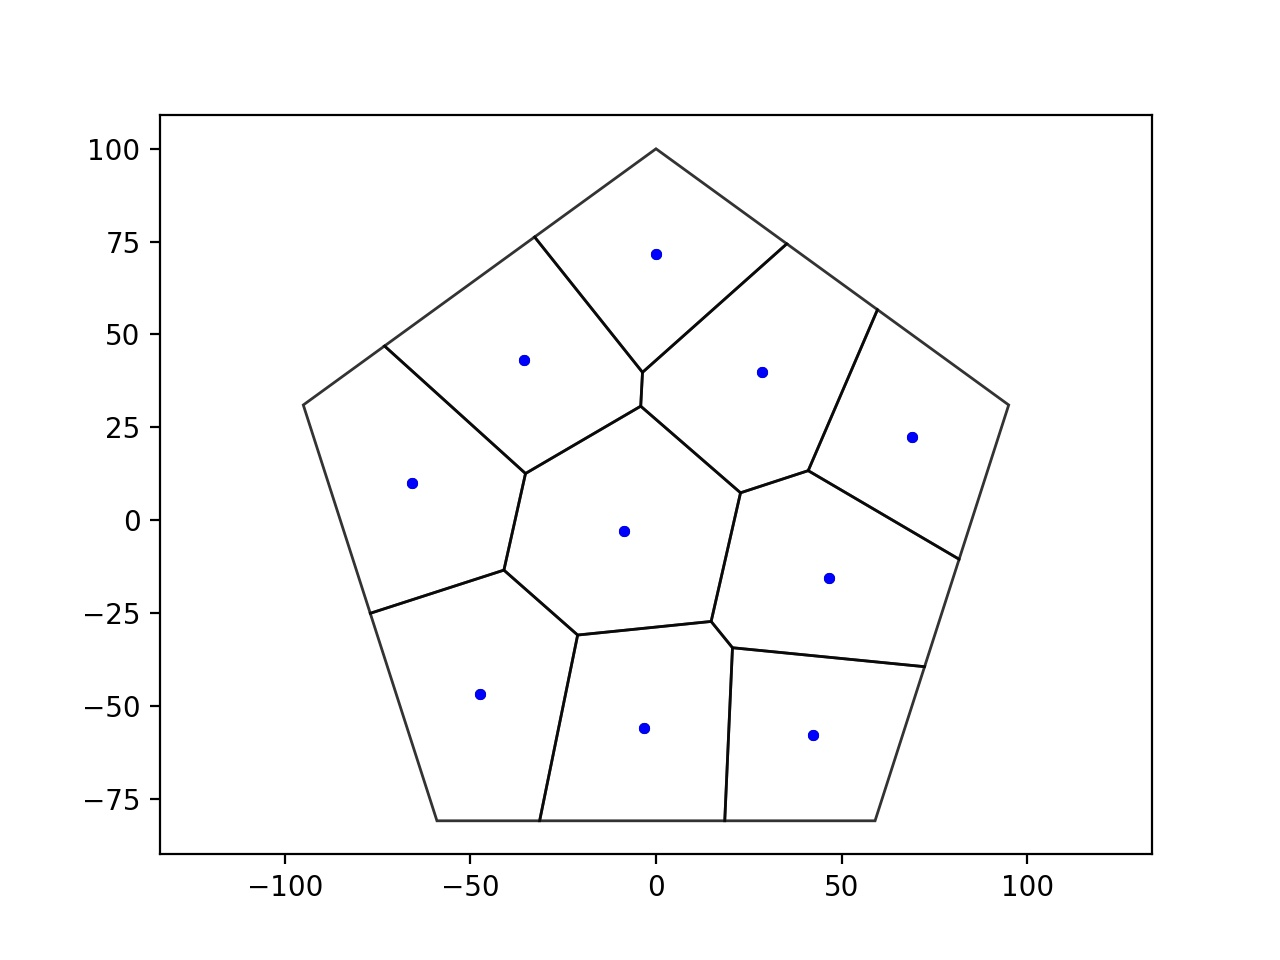
\includegraphics[scale=0.2]{voronoi_partition}
	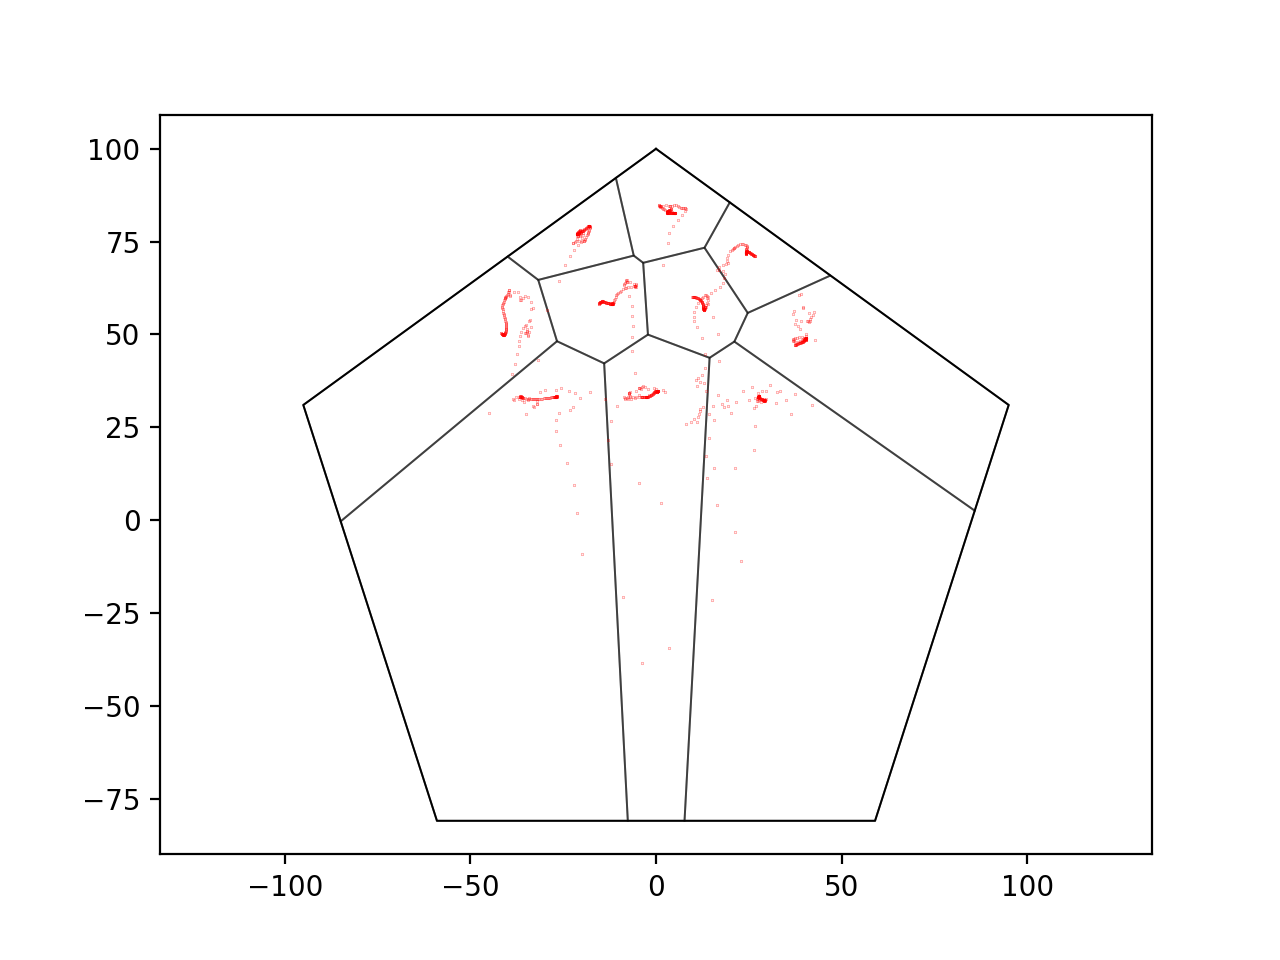
\includegraphics[scale=0.2]{gaussian_simulation_1}
}
{\sc\huge\bf Multi-Agent Area Coverage Control using Reinforcement Learning}	
{\Large \bf Adekunle Adepegba, Suruz Miah, Davide Spinello 
\\
Presented by Simon Hu}
% University logo
{
	\begin{tabular}{r}
		
\includegraphics[scale=0.5]{logo}
	\end{tabular}
}

\headerbox{Problem Statement}{name=problem_statement,column=0,row=0,span=1}
{
	Consider a group of $N$ homogeneous agents moving in a compact environment $\Omega \subset \R^2$ where the dynamics of the agent are given by $\dot{p_i} = g(p_i, u_i)$ where $p_i = (x_i, y_i) \in \R^2$ is the agent position and $u_i = (u_{x_i}, u_{y_i})$ represents the control input. The goal is to find a configuration of agent positions $p = (p_1, p_2, \dots, p_N$ such that the cost index
	\begin{equation*}
		\displaystyle \mathcal{H}(p, t) = \int_{\Omega}{\max\limits_{i=1,\dots,N}{f_i(\,\norm{p_i - q})} \phi(q, t) \dif q}
	\end{equation*}
	is maximized.
}
\headerbox{Voronoi Partitions}{name=cvp,below=problem_statement,span=1}
{
	The Voronoi partition of $\Omega$ is given by $\V = \bigcup \V_i$ where each $\V_i$ is given by 
	\begin{equation*}
		\displaystyle \left\{ q \in \Omega \: | \: \norm{q - p_i} \leq \norm{q - p_j}, \, \forall j \neq i \right\}.
	\end{equation*}
	The mass $m_{\V_i}$ and center of mass $c_{\V_i}$ of each $V_i$ are given by 
	\begin{equation*}
		\displaystyle m_{\V_i} = \int_{\V_i}{\phi \dif q}, c_{\V_i} = \frac{1}{m_{\V_i}}\int_{\V_i}{q\phi\dif q}
	\end{equation*}
	Then the cost index $\mathcal{H}$ can be rewritten as 
	\begin{equation*}
		\displaystyle \mathcal{H}(p, t) = \sum\limits_{i=1}^{n}{\int_{\V_i}{f_i(\,\norm{p_i - q}) \phi(q, t) \dif q}}.
	\end{equation*}
	\textrm{[Cort\'es et al., 2004]} showed that the optimal partition of $\Omega$ that maximizes $\mathcal{H}$ is the centroidal voronoi partition. 
	\begin{center}
		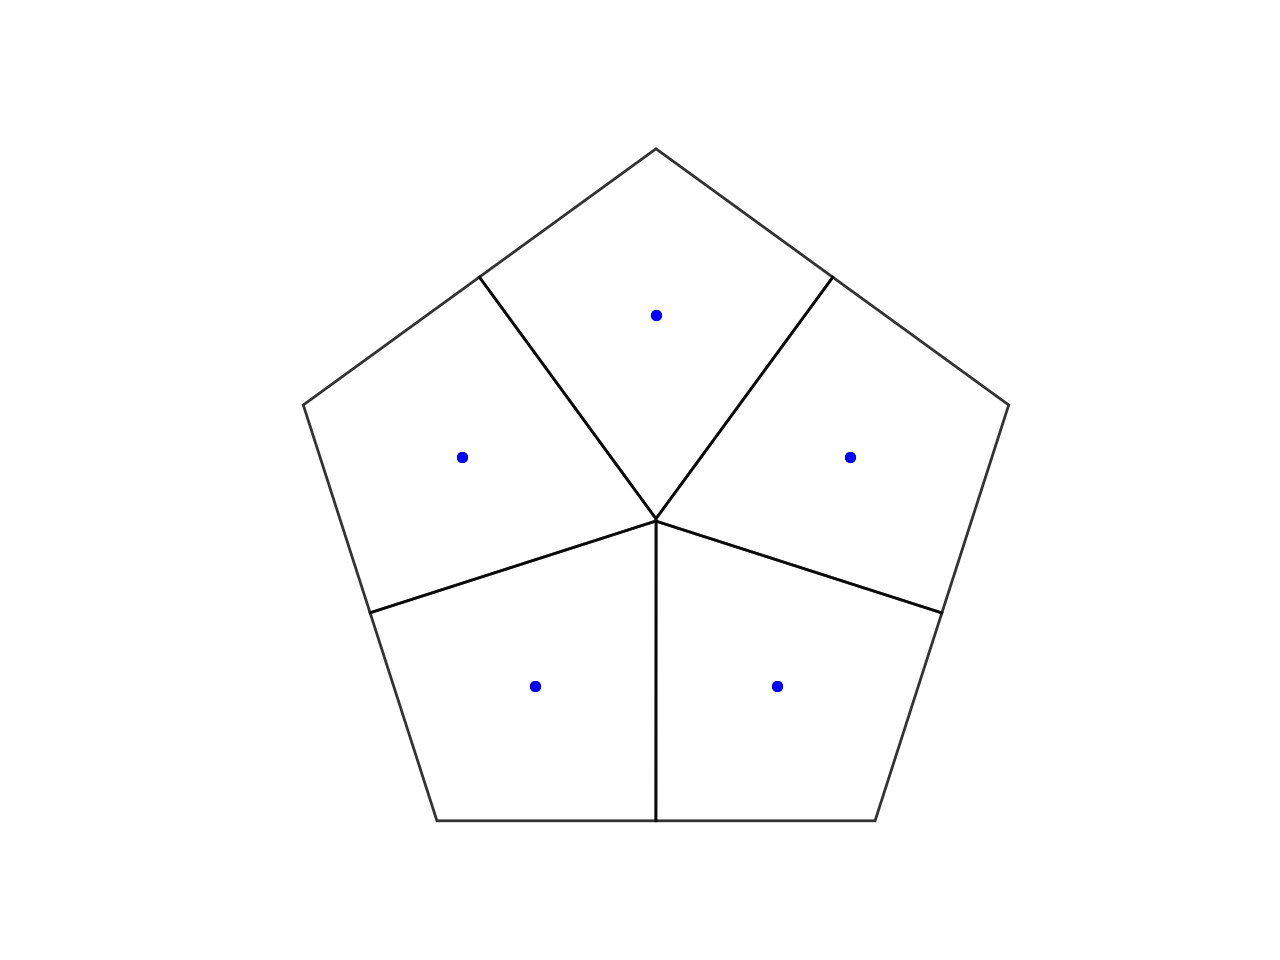
\includegraphics[scale=0.3]{fig_ex.png}
		\captionof{figure}{Example of a centroidal voronoi partition, for $\phi(q,t) = 1$.}
	\end{center}
}

\headerbox{TD3 Algorithm}{name=sacddpg,column=1,span=2}
{
	\begin{algorithm}[H]
		\caption{Twin-Delayed Actor-Critic DDPG}
		\begin{algorithmic}[1]
			\STATE Initialize critic networks $Q_{\theta_1}, Q_{\theta_2}$ and actor network $\pi_{\phi}$ with random parameters
			$\theta_1, \theta_2, \phi$. 
			\STATE Initialize the target networks $\theta'_1 \leftarrow \theta_1, \theta'_2 \leftarrow \theta_2, \phi' \leftarrow \phi$.
			\STATE Initialize a replay buffer $R$.
			\FOR {$t = 1$ \TO $T$}
				\STATE Select action with exploration noise $a \sim \pi(s) + \epsilon, \epsilon \sim \mathcal{N}(0, \sigma)$ and record the reward $r$ and new state $s'$. 
				\STATE Store the tuple $(s, a, r, s')$ into $R$. 
				\STATE Sample minibatches of $N$ transitions $(s, a, r, s')$ from $R$.
				\STATE Smooth the target policy according to $\tilde{a} \leftarrow \pi_{\phi'}(s) + \epsilon, \epsilon \sim \Clip(\mathcal{N}(0, \tilde{\sigma}), -c, c)$.
				\STATE Perform double $Q$-learning and clip the results according to $y \leftarrow r + \gamma \min_{1,2}Q_{\theta'_i}(s', \tilde{a})$. 
				\STATE Update the critics according to $\theta_i \leftarrow \min_{\theta_i}N^{-1}\sum(y - Q_{\theta_i}(s, a))^2$.
				\IF {$t \mod d$} 
					\STATE Update $\phi$ by the deterministic policy gradient $\nabla_{\phi}J(\phi) = N^{-1}\sum\nabla_a Q_{\theta_1}(s,a)\big|_{a = \pi_{\phi(s)}}\nabla_{\phi}\pi_{\phi(s)}$.
					\STATE Update the target networks according to $\theta'_i \leftarrow \tau\theta_i + (1-\tau)\theta'_i, \:\: \phi' \leftarrow \tau\phi + (1-\tau)\phi'$.
				\ENDIF 
			\ENDFOR
		\end{algorithmic}	
	\end{algorithm}

	The TD3 algorithm is an improvement on the SACDDPG algorithm, which is more vanilla, and prevents overestimation of the value function by decoupling the action selection and $Q$-value update. 
	\\ \\
	TD3 reduces variance by updating the policy at a lower frequency than the $Q$-function updates. 
	\\ \\
	A regularization strategy is introduced by adding a small amount of clipped random Gaussian noise to the selected action and then averages it over minibatches. 
}

\headerbox{Experimental Setup}{name=setup,column=3,span=2}
{
	Placeholder.
}

\headerbox{Results}{name=results,column=3,span=2,below=setup}
{
	Placeholder.
}

\headerbox{Extensions}{name=extentions,column=1,below=sacddpg,span=2}
{
	Placeholder.
}

\headerbox{}{name=references,column=3,span=2,below=results}
{
	\nocite{*}
	\bibliography{ref}
	\bibliographystyle{ieeetr}
}
\end{poster}
\end{document}